\documentclass[12pt, a4paper]{article}
%\documentclass[parskip,12pt,paper=a4,sffamily]{scrreprt}
%\usepackage[latin9]{inputenc}
%\usepackage[englisch, ngerman]{babel}
%%%%%%%%%%%%%%%%%%%%%%%%%%%%%%%%%%%%%%%%%%%%%%%%%%%%%%%%%%%%%%%%%%%%%%%%%%%%%%%
%%% FONT SETTING %%%
\usepackage[T1]{fontenc}
\usepackage[utf8]{inputenc}
%\usepackage[applemac]{inputenc}
\usepackage[onehalfspacing]{setspace}     % singlespacing
%\setstretch{1.3}                         % for other than standard spacings
%%%%%%%%%%%%%%%%%%%%%%%%%%%%%%%%%%%%%%%%%%%%%%%%%%%%%%%%%%%%%%%%%%%%%%%%%%%%%%%
%%% LAYOUT
\usepackage[left=3cm,top=2cm,right=3cm,nohead,nofoot]{geometry}
\setlength{\footskip}{2cm}      % Seitenzahl weiter n. unten, Achtung ggf. Problem bei Fussnoten
\setlength{\parindent}{0in}
\setlength{\parskip}{.1in}
\setlength{\textwidth}{140mm}
\setlength{\oddsidemargin}{10mm}
\usepackage[toc]{appendix}     % for named appendices
\usepackage{hanging}            % for hanging indent environment
%%%%%%%%%%%%%%%%%%%%%%%%%%%%%%%%%%%%%%%%%%%%%%%%%%%%%%%%%%%%%%%%%%%%%%%%%%%%%%%
%%% Subject index 
%\usepackage{makeidx}
%\makeindex{}
%\renewcommand{\indexname}{Subject index}      % change name of index page
%%%%%%%%%%%%%%%%%%%%%%%%%%%%%%%%%%%%%%%%%%%%%%%%%%%%%%%%%%%%%%%%%%%%%%%%%%%%%%%
%%% FIGURE AND TABLE SETTINGS %%%
\usepackage{booktabs}
\usepackage{subfigure}
\usepackage{rotating}
\usepackage{float}
\restylefloat{figure}     % H will mean directly here now
\usepackage[]{caption}   %bold caption label
\captionsetup[figure]{font=footnotesize, labelfont={footnotesize, bf}, labelsep=space}                                  % labelsep=newline
\captionsetup[table]{font=footnotesize, labelfont={footnotesize, bf}, labelsep=space}
\newcommand\T{\rule{0pt}{2.6ex}}          % global change toprule spaces table
\newcommand\B{\rule[-1.2ex]{0pt}{0pt}}    % global change bottomrule table
\setlength{\subfigtopskip}{5mm}           % set skips for subfigures and tables
\setlength{\subfigcapskip}{1mm}
%%%%%%%%%%%%%%%%%%%%%%%%%%%%%%%%%%%%%%%%%%%%%%%%%%%%%%%%%%%%%%%%%%%%%%%%%%%%%%%
%%% MATH
\usepackage{amsmath}
\usepackage{amssymb}
%%%%%%%%%%%%%%%%%%%%%%%%%%%%%%%%%%%%%%%%%%%%%%%%%%%%%%%%%%%%%%%%%%%%%%%%%%%%%%%
%%% HYPHENATIONS %%%
% \hyphenation{OpenRepGrid}       % no hyphenation in these words
%%%%%%%%%%%%%%%%%%%%%%%%%%%%%%%%%%%%%%%%%%%%%%%%%%%%%%%%%%%%%%%%%%%%%%%%%%%%%%%
%%% COMMANDS 
\title{Simulationen mit \R{}}
\author{Mark Heckmann} 

\newcommand{\code}[1]{\texttt{#1}}
\newcommand{\pkg}[1]{{\normalfont\fontseries{b}\selectfont #1}}
\newcommand{\R}{{\sffamily R}}

\usepackage[usenames]{color}  % nut rausnehmen wenn driver HighlightWeaveDriver aus highlight package genutzt wird, da dieser auch usepackage{color} einfügt
\definecolor{codecolor}{rgb}{0.400, 0.400, 0.400}


\usepackage{Sweave}
\begin{document} 
    
\maketitle

\begin{abstract}
Dieser Bericht soll Einsteigern anhand einiger Beispiel aufzeigen, wie mit \R{} Simulationen durchgeführt werden können.
\end{abstract}

\begin{singlespace}
\tableofcontents
\end{singlespace}
% Preface   

%%%%%%%%%%%%%%%%%%%%%%%%%%%%%%%%%%%%%%%%%%%%%%%%%%%%%%%%%%%%%%%%%%%%%%%%%%%%%%%
\newpage 
                                               %%%%%%%%%%%%%%%%%%%%%%%%%%%%%%%%%%%%%%%%%%%%%%%%%%%%%%%%%%%%%%%%%%%%%%%%%%%%%%%
%%% SWEAVE
       % Ihaka, R. (2009). Customizing Sweave 
%%%%%%%%%%%%%%%%%%%%%%%%%%%%%%%%%%%%%%%%%%%%%%%%%%%%%%%%%%%%%%%%%%%%%%%%%%%%%%%
%%% CUSTOMIZING SWEAVE 
%%% from: Ihaka, R. (2009). Customizing Sweave to Produce Better Looking LATEX Output
\DefineVerbatimEnvironment{Sinput}{Verbatim}{fontsize=\footnotesize, formatcom=\color{codecolor}, xleftmargin=2em}
\DefineVerbatimEnvironment{Soutput}{Verbatim}{fontsize=\footnotesize, xleftmargin=2em, formatcom=\color{codecolor}} 
\DefineVerbatimEnvironment{Scode}{Verbatim}{fontsize=\footnotesize, xleftmargin=2em, formatcom=\color{codecolor}}

\renewenvironment{Schunk}{\vspace{10pt}}{\vspace{8pt}}   
%%%%%%%%%%%%%%%%%%%%%%%%%%%%%%%%%%%%%%%%%%%%%%%%%%%%%%%%%%%%%%%%%%%%%%%%%%%%%%%
%%%%%%%%%%%%%%%%%%%%%%%%%%%%%%%%%%%%%%%%%%%%%%%%%%%%%%%%%%%%%%%%%%%%%%%%%%%%%%%

\section{Stichprobenverteilung des Mittelwerts}

\begin{Schunk}
\begin{Sinput}
> mu <- 100
> s <- 10
> pop <- rnorm(1e3, mu, s)
> hist(pop, breaks=40, col="grey")
\end{Sinput}
\end{Schunk}
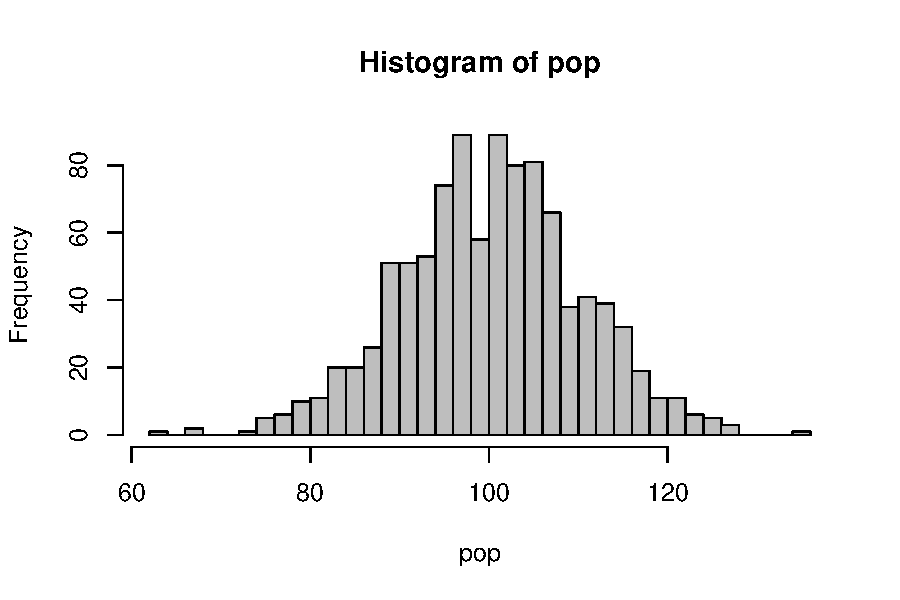
\includegraphics{sim_mean_dist-002}


\begin{Schunk}
\begin{Sinput}
> sample_means <- function(pop, n, nrep=1000){
   res <- rep(NA, nrep)
   for (i in 1:nrep)
     res[i] <- mean(sample(pop, n))  
   res
 }
\end{Sinput}
\end{Schunk}

\begin{Schunk}
\begin{Sinput}
> ns <- seq(10, 200, 40)
> l <- list()
> for (i in seq_along(ns)){
   means <- sample_means(pop, ns[i])
   l[[i]] <- data.frame(n=ns[i], means)  
 }       
> x <- do.call(rbind, l)
\end{Sinput}
\end{Schunk}

\begin{Schunk}
\begin{Sinput}
> library(ggplot2)
> ggplot(x, aes(x=means)) + geom_histogram(binwidth=.2) +
   facet_grid(. ~ n)
\end{Sinput}
\end{Schunk}
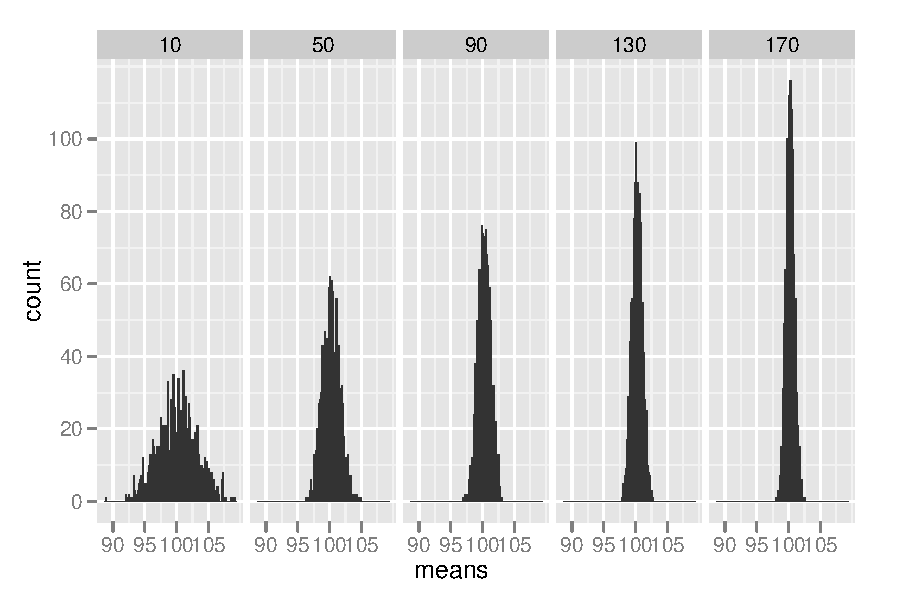
\includegraphics{sim_mean_dist-005}











\newpage 
                                               %%%%%%%%%%%%%%%%%%%%%%%%%%%%%%%%%%%%%%%%%%%%%%%%%%%%%%%%%%%%%%%%%%%%%%%%%%%%%%%
%%% SWEAVE
       % Ihaka, R. (2009). Customizing Sweave 
%%%%%%%%%%%%%%%%%%%%%%%%%%%%%%%%%%%%%%%%%%%%%%%%%%%%%%%%%%%%%%%%%%%%%%%%%%%%%%%
%%% CUSTOMIZING SWEAVE 
%%% from: Ihaka, R. (2009). Customizing Sweave to Produce Better Looking LATEX Output
\DefineVerbatimEnvironment{Sinput}{Verbatim}{fontsize=\footnotesize, formatcom=\color{codecolor}, xleftmargin=2em}
\DefineVerbatimEnvironment{Soutput}{Verbatim}{fontsize=\footnotesize, xleftmargin=2em, formatcom=\color{codecolor}} 
\DefineVerbatimEnvironment{Scode}{Verbatim}{fontsize=\footnotesize, xleftmargin=2em, formatcom=\color{codecolor}}

\renewenvironment{Schunk}{\vspace{10pt}}{\vspace{8pt}}   
%%%%%%%%%%%%%%%%%%%%%%%%%%%%%%%%%%%%%%%%%%%%%%%%%%%%%%%%%%%%%%%%%%%%%%%%%%%%%%%
%%%%%%%%%%%%%%%%%%%%%%%%%%%%%%%%%%%%%%%%%%%%%%%%%%%%%%%%%%%%%%%%%%%%%%%%%%%%%%%


\section{Varianzschätzung}

Die Definition der Varianz einer Zufallsvariable $X$ ist wohlbekannt. 

\begin{equation}
\operatorname{Var}(X) = \operatorname{E}\left( (X-\mu)^2\right)  
\end{equation}  

Sie berechnet sich wie folgt, wenn der wahre Mittelwert $\mu$ der Variablen $X$ bekannt ist. 

\begin{equation} \label{eq:var_mu}
  \sigma^2 = \frac{\sum{(x_i - \mu)^2}}{n}  
\end{equation}

Dies ist jedoch in der Regel nicht der Fall, so dass $\bar x$ geschätzt werden muss. So könnte man $\mu$ wird dann durch diesen Schätzwert ersetzen.

\begin{equation} \label{eq:var_mean}
  S^2 = \frac{\sum{(x_i - \bar x)^2}}{n}  
\end{equation} 

Hierbei handelt es sich jedoch nicht mehr um eine erwartungstreue Schätzung der Varianz von $X$. Dass dies nicht der Fall ist, soll nachfolgend simuliert werden. Hierzu programmieren wir zwei Funktionen. Eine die den Populationsmittelwert (Formel \ref{eq:var_mu}) und eine die den Stichprobenmittelwert(Formel \ref{eq:var_mean}) zur Schätzung der Varianz nutzt.  


\begin{Schunk}
\begin{Sinput}
> var_mu <- function(x, mu){   
   sum((x - mu)^2) / length(x)  
 }   
> var_mean <- function(x){
   xm <- mean(x)
   sum((x - xm)^2) / length(x)
 }
> x <- rnorm(1e3, 100, 10)
> var_mu(x, 100)  
\end{Sinput}
\begin{Soutput}
[1] 99.52682
\end{Soutput}
\begin{Sinput}
> var_mean(x)
\end{Sinput}
\begin{Soutput}
[1] 99.50176
\end{Soutput}
\end{Schunk}

Wir sehen, dass zwischen den beiden Schätzern Unterschiede bestehen können. An diesem Punkt ist es jedoch schwer zu sagen, ob diese Unterschiede einen Einfluss auf die Güte der Schätzung haben könnten. Aus diesem Grund simulieren wir viele Stichprobenziehungen.

\begin{Schunk}
\begin{Sinput}
> compare_est <- function(nrep, n, mu, s){
   res.mu <- rep(NA, nrep)         # Ergebnisvektor mu
   res.mean <- rep(NA, nrep)       # Ergebnisvektor mean
   counter <- 1                    # Zähler
   for (i in 1:nrep){
     cat("\r run", i)              # Ausgabe Durchlauf
     flush.console()               # Zwischenspeicher entleeren
     x <- rnorm(n, mu, s)          # Stichprobe ziehen
     res.mu[i] <- var_mu(x, mu)    # Varianzschätzung mu
     res.mean[i] <- var_mean(x)    # Varianzschätzung mean
     counter <- counter + 1        # Zähler erhöhen 
   }
   c(var.mu= mean(res.mu),         # mu und mean Schätzung
     var.mean=mean(res.mean))      # ausgeben
 }
> compare_est(1e3, 100, 100, 10)
\end{Sinput}
\end{Schunk}

\begin{Schunk}
\begin{Soutput}
   var.mu  var.mean 
100.17497  99.16071 
\end{Soutput}
\end{Schunk}

Um eine besser Aussage treffen zu können simulieren wir die Daten erneut für verschiedene Stichprobenumfänge $n$.

\begin{Schunk}
\begin{Sinput}
> ns <- seq(10, 100, 10)              # verschiedene n
> len.ns <- length(ns)                # Anzahl an n Werten
> rmat <- matrix(NA, len.ns, 2)       # Ergebnismatrix initialisieren
> for (i in 1:len.ns)
   rmat[i, ] <- compare_est(1e3, ns[i], 100, 10)    
> r <- as.data.frame(rmat)            # in dataframe verwandeln
> names(r) <- c("var.mu", "var.mean") # Spalten benennen
> r <- cbind(n=ns, r)                 # n Spalte hinzufügen
> r
\end{Sinput}
\begin{Soutput}
     n    var.mu var.mean
1   10 100.06657 89.64241
2   20  98.76847 94.02082
3   30  99.60366 96.19998
4   40  99.52436 96.90844
5   50  99.72247 97.70548
6   60 100.09744 98.45187
7   70 100.02446 98.57086
8   80  99.15451 97.92934
9   90  99.76741 98.58419
10 100 100.86990 99.94020
\end{Soutput}
\end{Schunk}

Es wird deutlich, dass die Schätzfunktion auf Basis der Mittelwertes die Varianz systematisch unterschätzt. Formel \ref{eq:var_mean} liefert somit keine erwartungstreue Schätzung von $\sigma^2$. Mit steigendem $n$ näheren sich die Schätzer jedoch an.  Welcher Zusammenhang besteht hierbei zwischen den beiden Schätzern? 

\begin{Schunk}
\begin{Sinput}
> r <- transform(r, diff=var.mu - var.mean)
> r <- transform(r, n_diff=n * diff) 
> r
\end{Sinput}
\begin{Soutput}
     n    var.mu var.mean       diff    n_diff
1   10 100.06657 89.64241 10.4241538 104.24154
2   20  98.76847 94.02082  4.7476497  94.95299
3   30  99.60366 96.19998  3.4036721 102.11016
4   40  99.52436 96.90844  2.6159222 104.63689
5   50  99.72247 97.70548  2.0169902 100.84951
6   60 100.09744 98.45187  1.6455749  98.73450
7   70 100.02446 98.57086  1.4536003 101.75202
8   80  99.15451 97.92934  1.2251662  98.01329
9   90  99.76741 98.58419  1.1832200 106.48980
10 100 100.86990 99.94020  0.9296927  92.96927
\end{Soutput}
\end{Schunk}

Die Differenz zwischen den Schätzfunktionen scheint systematisch mit $n$ zusammenzuhängen.

Um aus Formel \ref{eq:var_mean} einen erwartungstreuen Schätzer zu machen muss diese um eine Korrekturfaktor $\frac{n}{n-1}$ erweitert werden. 

\begin{Schunk}
\begin{Sinput}
> transform(r, corr.var.mean=var.mean *n / (n-1))
\end{Sinput}
\begin{Soutput}
     n    var.mu var.mean       diff    n_diff corr.var.mean
1   10 100.06657 89.64241 10.4241538 104.24154      99.60268
2   20  98.76847 94.02082  4.7476497  94.95299      98.96928
3   30  99.60366 96.19998  3.4036721 102.11016      99.51723
4   40  99.52436 96.90844  2.6159222 104.63689      99.39327
5   50  99.72247 97.70548  2.0169902 100.84951      99.69946
6   60 100.09744 98.45187  1.6455749  98.73450     100.12054
7   70 100.02446 98.57086  1.4536003 101.75202      99.99942
8   80  99.15451 97.92934  1.2251662  98.01329      99.16895
9   90  99.76741 98.58419  1.1832200 106.48980      99.69188
10 100 100.86990 99.94020  0.9296927  92.96927     100.94970
\end{Soutput}
\end{Schunk}

Die erwartungstreue Varianzschätzung auf Basis einer Stichprobe ist somit

\begin{eqnarray} \label{eq:var_sample}
  S^2 &=& \frac{n}{n-1} \frac{\sum{(x_i - \bar x)^2}}{n} \\  
           &=& \frac{\sum{(x_i - \bar x)^2}}{n-1}.
\end{eqnarray}

\par
\textbf{Berechnung mit Funktionen aus der \texttt{apply}-Familie}  

Alternativ zu eienr Schliefe können auch Funktionen der \texttt{apply}-Familie genutzt werden. 

\begin{Schunk}
\begin{Sinput}
> compare_est_2 <- function(reps, n, mu, s){
   x <- replicate(reps, rnorm(n, mu, s))
   vars_mu <- apply(x, 2, var_mu, mu)
   vars_mean <- apply(x, 2, var_mean)
   c(var.mu= mean(vars_mu),              # mu und mean Schätzung
     var.mean=mean(vars_mean))           # ausgeben  
 }
> compare_est_2(1e3, 100, 100, 10)
\end{Sinput}
\begin{Soutput}
   var.mu  var.mean 
100.03783  99.14195 
\end{Soutput}
\begin{Sinput}
> ns <- seq(10, 100, 10)
> res <- mapply(compare_est_2, reps=1e3, n=ns, mu=100, s=10)
> r <- as.data.frame(t(res))              # in dataframe verwandeln
> r <- cbind(n=ns, r)                     # n Spalte hinzufügen
> r
\end{Sinput}
\begin{Soutput}
     n    var.mu  var.mean
1   10 100.34796  90.62385
2   20  99.49068  94.46534
3   30 100.57160  97.18186
4   40 100.09461  97.59578
5   50 100.57407  98.45921
6   60  99.39860  97.71116
7   70 100.14886  98.77468
8   80 101.30143 100.00589
9   90  99.82390  98.69558
10 100  99.73707  98.80649
\end{Soutput}
\end{Schunk}


\textbf{Die analytische Herleitung der korrigierten Stichprobenvarianz}

\begin{align} 
    E (S_1^2)  &= \frac 1n \sum_{i=1}^n E\left( (X_i-\overline{X})^2 \right)= 
  \frac 1n E \left(\sum_{i=1}^n (X_i-\mu+\mu-\overline{X})^2\right)\\
  &=\frac1n E \left(\sum_{i=1}^n \left((X_i-\mu)^2 - 2(X_i-\mu)
  (\overline{X}-\mu) + (\overline{X}-\mu)^2\right) \right)\\
  &=\frac1n E\left(\sum_{i=1}^n (X_i-\mu)^2 - 2\sum_{i=1}^n(X_i-\mu)
  (\overline{X}-\mu) + n(\overline{X}-\mu)^2\right) \\
  &=\frac1n E\left(\sum_{i=1}^n (X_i-\mu)^2 - 2n(\overline{X}-\mu)
  (\overline{X}-\mu) + n(\overline{X}-\mu)^2\right) \\
  &=\frac1n E\left(\sum_{i=1}^n (X_i-\mu)^2 -n(\overline{X}-\mu)^2\right) \\
  &=\frac1n \left(\sum_{i=1}^n E\left((X_i-\mu)^2\right) -nE\left((\overline{X}-\mu)^2\right)\right) \\
  &=\frac1n \left(nVar(X)-nVar(\overline{X})\right) \\
  &=Var(X)-Var(\overline{X}) = \sigma^2 - \frac{\sigma^2}{n} = \frac{n-1}{n}\,\sigma^2, \end{align} 


 




%%%%%%%%%%%%%%%%%%%%%%%%%%%%%%%%%%%%%%%%%%%%%%%%%%%%%%%%%%%%%%%%%%%%%%%%%%%%%%%
   
\newpage
%%%%%%%%%%%%%%%%%%%%%%%%%%%%%%%%%%%%%%%%%%%%%%%%%%%%%%%%%%%%%%%%%%%%%%%%%%%%%%%

\section{$\Pi$ berechnen}

Wir stellen uns die Frage, in welchem Verhältnis die Fläche eines Qudrates zu der Fläche des in dieses Quadrat eingeschriebenen Kreises ist. 

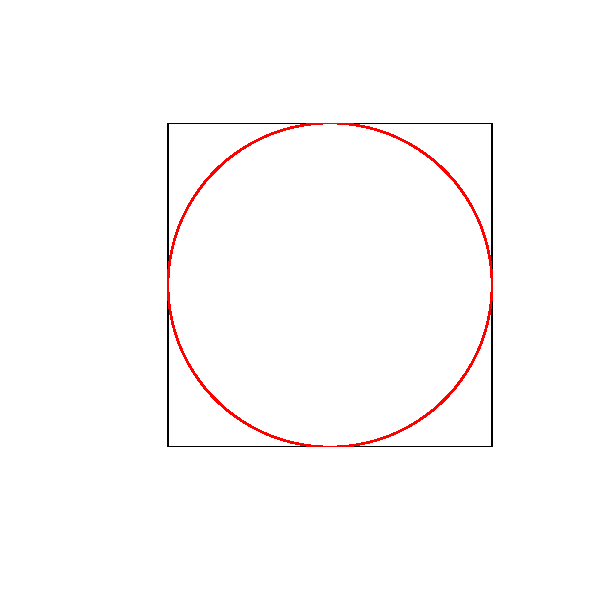
\includegraphics{sim_pi-001}

Die Kantenlänge des Quadrates sei $2r=2$ somit hat der Kreis den Radius $r=1$. Die Fläche des Kreises ist folglich $\pi r^2 = \pi 1^2 = \pi$. Die Fläche des Quadrats ist $(2r)^2=4$. Das Verhältnis der beiden Flächen zueinander ist somit:

\begin{equation} \label{eq:pi}
  \rho = \frac{\text{Fläche des Kreises}}{\text{Fläche des Quadrats}} = \frac{\pi r^2}{(2r)^2} = \frac{\pi}{4}
\end{equation}

Die Herangehensweise ist nun zufällig Punkte innerhlab des Quadrates zu erzeugen. Im nächten Schritt werden die Punkte, die innerhalb und außerhalb des Kreises fallen ausgezählt Das Verhätnis zwischen ihnen multipliziert mit 4 ist eine Schätzung von $\pi$.
Um die Punkte innerhlab des Kreieses zu bestimmen berechnen wir ihren Abstand vom Zentrum. Dieser darf maximal $1$ betragen.

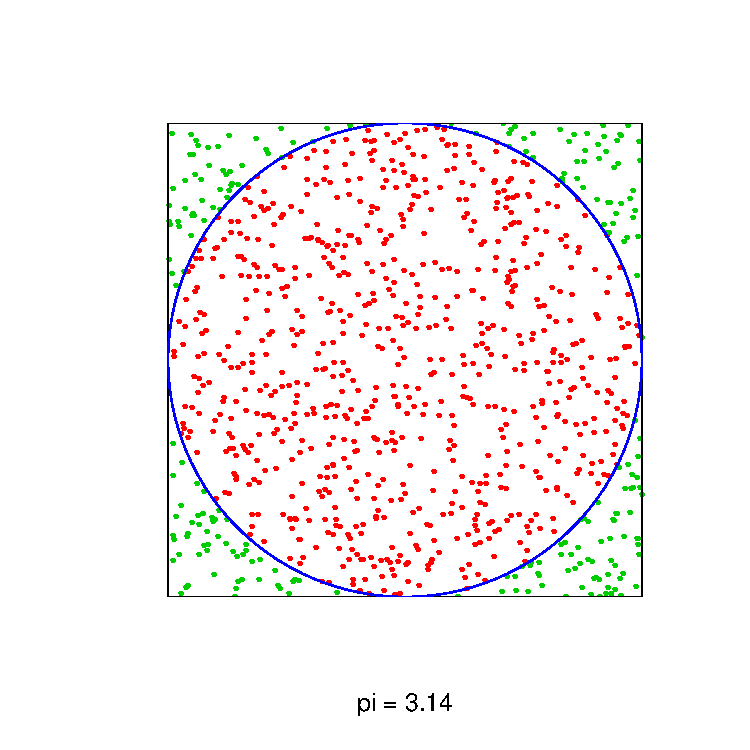
\includegraphics{sim_pi-002}

Berechnen wir nun dieses Verhältnis für eine größere Anzahl an Punkten. Um den Abstand von Zentrum zu berechnen wird die euklidische Distanz genutzt, $\sqrt{x^2 + y^2}$. Alle Punkte mit einer Distanz kleiner gleich Eins liegen innerhalb des Kreises.
          
\begin{Schunk}
\begin{Sinput}
> estimate_pi <- function(n=10e4){
+   x <- runif(n, -1, 1)                # Zufällige x Werte 
+   y <- runif(n, -1, 1)                # Zufällige y Werte
+   z <- sqrt(x^2 + y^2)                # Abstand zum Ursprung
+   n.in.circle <- length(z[z <= 1])    # Anzahl an Punkten im Kreis
+   n.in.circle / n * 4                 # Verhältnis * 4
+ } 
> estimate_pi(10e4)
\end{Sinput}
\begin{Soutput}
[1] 3.13904
\end{Soutput}
\end{Schunk}

Die Schätzung funktioniert. Der letzte Schritt in eier Simulation ist es häufig den Code schneller zu machen. In unseren Fall ist dies nciht wichtig, da die Simulation nur wenige Sekunden dauert. Bei längeren Simulationen könne so jedoch Stunden oder gar Tage an Rechenzeit eingespart werden. Unser Ziel ist es hier, alle Operationen, die nicht nötig sind wegzulassen. Um die Laufzeit der Simulation zu überpfüfen kann die Funktion \texttt{system.time} genutzt werden.

\begin{Schunk}
\begin{Sinput}
> system.time({
+   estimate_pi(10e5)
+ })   
\end{Sinput}
\begin{Soutput}
   user  system elapsed 
  0.161   0.056   0.256 
\end{Soutput}
\end{Schunk}

Nehmen wir nun eineige Verbessrungen vor. Da wir nur wissen wollen, welche Werte kleiner oder gleich Eins sind ist die Wurzeloperation nicht nötig. Darüber hinaus kann auch beim Auszählen der Punkte im Kreis eine Operation gespart werden.

\begin{Schunk}
\begin{Sinput}
> estimate_pi_2 <- function(n=10e4){
+   x <- runif(n, -1, 1)
+   y <- runif(n, -1, 1) 
+   z <- x^2 + y^2                    # keine Wurzel
+   n.in.circle <- sum(z <= 1)        # kein Vektorzugriff 
+   n.in.circle / n * 4  
+ } 
\end{Sinput}
\end{Schunk}

\begin{Schunk}
\begin{Sinput}
> system.time({
+   estimate_pi_2(10e5)
+ })   
\end{Sinput}
\begin{Soutput}
   user  system elapsed 
  0.132   0.037   0.235 
\end{Soutput}
\end{Schunk}

Die Performance hat sich durch diese Schritte um gut $25\,\%$ verbessert. Eliminieren wir zuletzt noch einige unnötige Speicherschritte.

\begin{Schunk}
\begin{Sinput}
> estimate_pi_3 <- function(n=10e4){ 
+   z <- runif(n, -1, 1)^2 + 
+        runif(n, -1, 1)^2
+   sum(z <= 1) / n * 4 
+ } 
\end{Sinput}
\end{Schunk}

\begin{Schunk}
\begin{Sinput}
> system.time({
+   estimate_pi_3(10e6)
+ })   
\end{Sinput}
\begin{Soutput}
   user  system elapsed 
  1.469   0.446   2.497 
\end{Soutput}
\end{Schunk}

Die Performance hat sich so erneut um ca. $20\,\%$ verbessert. 

%%%%%%%%%%%%%%%%%%%%%%%%%%%%%%%%%%%%%%%%%%%%%%%%%%%%%%%%%%%%%%%%%%%%%%%%%%%%%%%
    
\newpage
                                               %%%%%%%%%%%%%%%%%%%%%%%%%%%%%%%%%%%%%%%%%%%%%%%%%%%%%%%%%%%%%%%%%%%%%%%%%%%%%%%
%%% SWEAVE
       % Ihaka, R. (2009). Customizing Sweave 
%%%%%%%%%%%%%%%%%%%%%%%%%%%%%%%%%%%%%%%%%%%%%%%%%%%%%%%%%%%%%%%%%%%%%%%%%%%%%%%
%%% CUSTOMIZING SWEAVE 
%%% from: Ihaka, R. (2009). Customizing Sweave to Produce Better Looking LATEX Output
\DefineVerbatimEnvironment{Sinput}{Verbatim}{fontsize=\footnotesize, formatcom=\color{codecolor}, xleftmargin=2em}
\DefineVerbatimEnvironment{Soutput}{Verbatim}{fontsize=\footnotesize, xleftmargin=2em, formatcom=\color{codecolor}} 
\DefineVerbatimEnvironment{Scode}{Verbatim}{fontsize=\footnotesize, xleftmargin=2em, formatcom=\color{codecolor}}

\renewenvironment{Schunk}{\vspace{10pt}}{\vspace{8pt}}   
%%%%%%%%%%%%%%%%%%%%%%%%%%%%%%%%%%%%%%%%%%%%%%%%%%%%%%%%%%%%%%%%%%%%%%%%%%%%%%%
%%%%%%%%%%%%%%%%%%%%%%%%%%%%%%%%%%%%%%%%%%%%%%%%%%%%%%%%%%%%%%%%%%%%%%%%%%%%%%%

\section{Stichprobenverteilung von Korrelationskoeffizienten}

Signifikanstests und Konfodenzintervalle für Korrelationskoeffizeinten werden mit Hilfe von Fisher's Z-Transformation berechnet (nichts zu verwechselen mit der z-Transormation). Sie hat folgende Form.

\begin{equation} \label{eq:fisher}
  f(\varrho)=0{,}5\ln\left(\frac{1+\varrho}{1-\varrho}\right)  
\end{equation}                                               

\begin{Schunk}
\begin{Sinput}
> fisher.z <- function(r){
   .5 * log((1+r) / (1-r))
 }
\end{Sinput}
\end{Schunk}

% \begin{equation}
% z_1=f(r)-\frac{z_{1-\alpha/2}}{\sqrt{n-3}} \leq\mu\leq f(r)+\frac{z_{1-\alpha/2}}{\sqrt{n-3}}=z_2     
% \end{equation}  

Warum ist dies nötig und was bewirkt sie? Um dies besser zu verstehen sollen Korrelationskoeffizienten aus unterschielichen Populationen simuliert werden.

\begin{Schunk}
\begin{Sinput}
> sim_pop <- function(r, n=1000){
   x1 <- rnorm(n)
   x3 <- rnorm(n)
   x2 <- r * x1 + sqrt(1 - r^2) * x3
   data.frame(x1, x2) 
 }
> mean(replicate(1000, cor(sim_pop(.5))[1,2]))
\end{Sinput}
\begin{Soutput}
[1] 0.4999013
\end{Soutput}
\end{Schunk}

Die Daten werden korrekt erstellt. Um einen Eindruck von der Stichprobenverteilung von Korrelationskoeffizeinten zu bekommen erzeigen wir eine Population und ziehen aus dieser wiederholt eine Stichprobe auf dessen Basis wir die Korrelation errechnen.

\begin{Schunk}
\begin{Sinput}
> sample_dist <- function(r, n, nrep){
   x <- sim_pop(r, 1e5)
   res <- rep(NA, nrep)
   for (i in 1:nrep){
     index <- sample(1:nrow(x), n)
     res[i] <- cor(x[index, 1], x[index, 2])  
   }
   res  
 }
\end{Sinput}
\end{Schunk}

\begin{Schunk}
\begin{Sinput}
> x <- sample_dist(0, 100, 1e3)
> hist(x, breaks=40, xlim=c(-.5,1))  
\end{Sinput}
\end{Schunk}
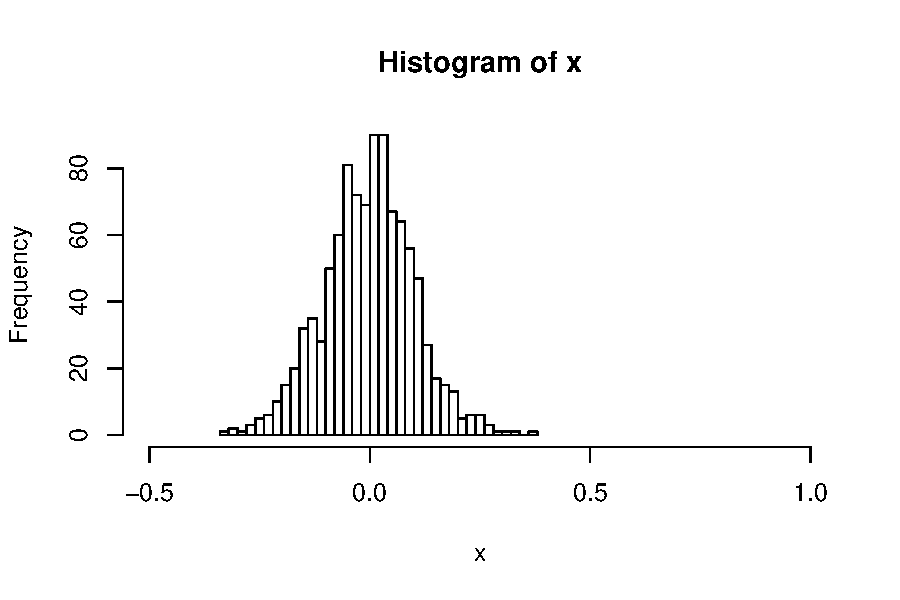
\includegraphics{sim_correlation-005}

Die Verteilung ist symmetrisch und errinnert an eine Gauß-Verteilung.
Die Wiederholen wir den Vorgang mit 

\begin{Schunk}
\begin{Sinput}
> x <- sample_dist(.7, 100, 1e3)
> hist(x, breaks=40, xlim=c(-.5,1))  
\end{Sinput}
\end{Schunk}
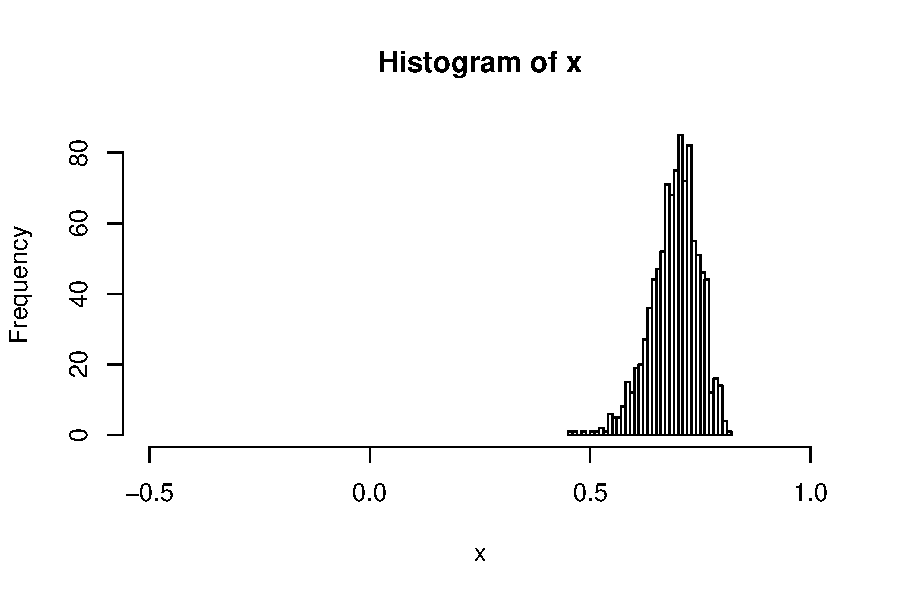
\includegraphics{sim_correlation-006}

Um dies besser zu verstehen simulieren wir Verteilungen für diverse $r$.
\begin{Schunk}
\begin{Sinput}
> r <- numeric()
> rpops <- seq(.3, .9, .2)
> for (i in seq_along(rs))
   r <- c(r, sample_dist(rpops[i], 100, 1000))
> rpop <- rep(rpops, each=1000)
> rz <- fisher.z(r)
> xr <- data.frame(rpop, r=r) 
> xz <- data.frame(rpop, r=rz) 
\end{Sinput}
\end{Schunk}

\begin{Schunk}
\begin{Sinput}
> library(ggplot2)
> g <- ggplot(xr, aes(x=r), ) +  geom_density() + 
             facet_grid(. ~ rpop)
> g
\end{Sinput}
\end{Schunk}
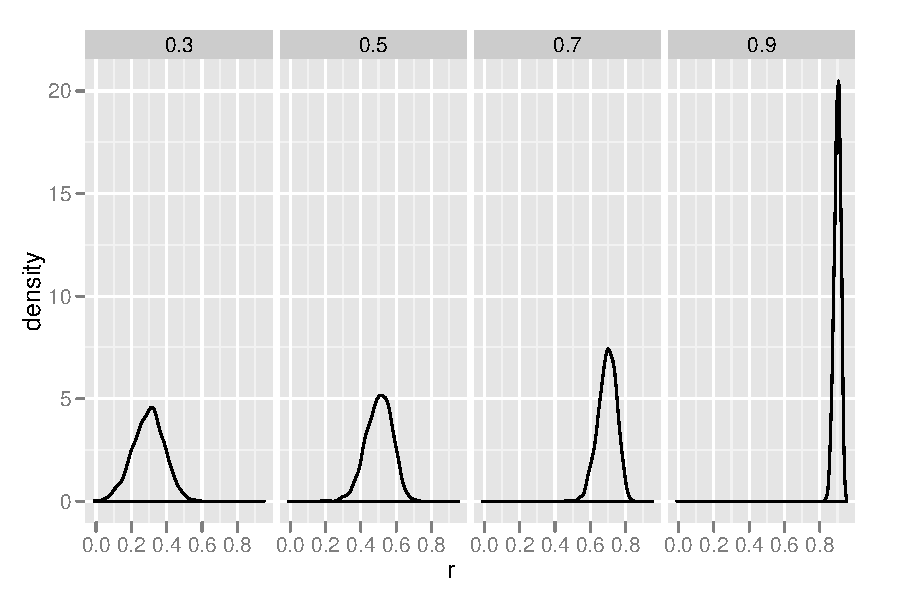
\includegraphics{sim_correlation-008}

\begin{Schunk}
\begin{Sinput}
> g %+% xz
\end{Sinput}
\end{Schunk}
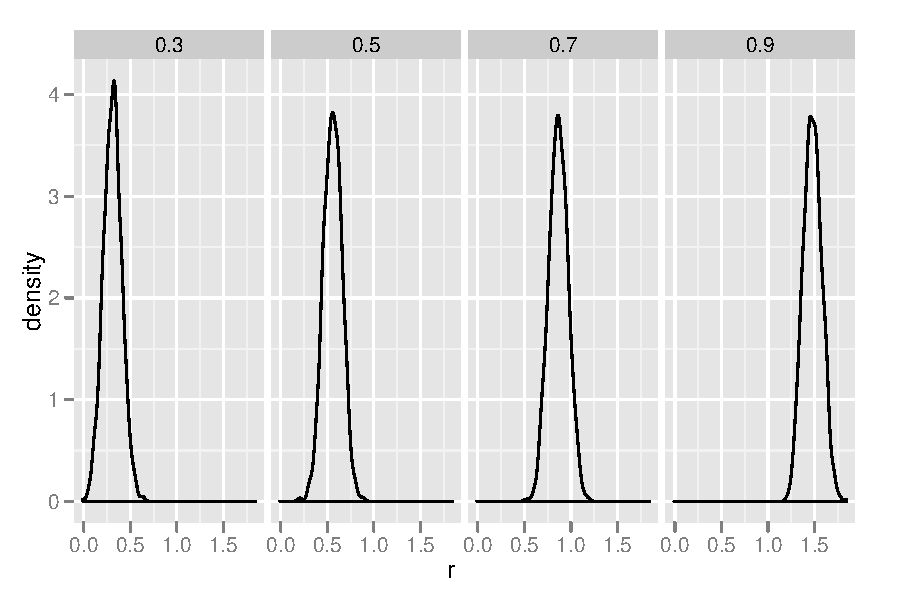
\includegraphics{sim_correlation-009}







\newpage 
              %%%%%%%%%%%%%%%%%%%%%%%%%%%%%%%%%%%%%%%%%%%%%%%%%%%%%%%%%%%%%%%%%%%%%%%%%%%%%%%
%%% SWEAVE
       % Ihaka, R. (2009). Customizing Sweave 
%%%%%%%%%%%%%%%%%%%%%%%%%%%%%%%%%%%%%%%%%%%%%%%%%%%%%%%%%%%%%%%%%%%%%%%%%%%%%%%
%%% CUSTOMIZING SWEAVE 
%%% from: Ihaka, R. (2009). Customizing Sweave to Produce Better Looking LATEX Output
\DefineVerbatimEnvironment{Sinput}{Verbatim}{fontsize=\footnotesize, formatcom=\color{codecolor}, xleftmargin=2em}
\DefineVerbatimEnvironment{Soutput}{Verbatim}{fontsize=\footnotesize, xleftmargin=2em, formatcom=\color{codecolor}} 
\DefineVerbatimEnvironment{Scode}{Verbatim}{fontsize=\footnotesize, xleftmargin=2em, formatcom=\color{codecolor}}

\renewenvironment{Schunk}{\vspace{10pt}}{\vspace{8pt}}   
%%%%%%%%%%%%%%%%%%%%%%%%%%%%%%%%%%%%%%%%%%%%%%%%%%%%%%%%%%%%%%%%%%%%%%%%%%%%%%%
%%%%%%%%%%%%%%%%%%%%%%%%%%%%%%%%%%%%%%%%%%%%%%%%%%%%%%%%%%%%%%%%%%%%%%%%%%%%%%%

\section{Formel für Konfidenzintervalle für binomiale Anteile überprüfen}

Nehmen wir haben in einer Umfrage mit $n=500$ Personen erfragt, ob sie die FDP wählen würden, wenn kommenden Sonntag Bundestagswahl wäre. $5\%$ der Befragten gaben an, dass sie die Partei wählen würden. Wie groß ist das Konfidenzinterval? In vielen Statistikehrbüchern wird folgenden Formel für die Berechnung der Konfidenzintervalle für binomiale Anteilswerte aufgeführt. 

\begin{equation} \label{eq:prop_standard}
\hat p + z_{1- \frac{\alpha}{2}} \cdot \frac{\sqrt{\hat p(1-\hat p)}}{\sqrt{n}}
\end{equation}

% \begin{eqnarray} \label{eq:prop_standard_2}
% c = \Phi^{-1} \left( 1 - {\alpha \over 2} \right) \\
% p_u = \hat p - c \cdot \sqrt{\hat p \cdot (1-\hat p) \over n} \\
% p_o = \hat p + c \cdot \sqrt{\hat p \cdot (1-\hat p) \over n} 
% \end{eqnarray}   
  
Schreiben wir hierzu in \R{} eine Funktion, die dies berechnet.

\begin{Schunk}
\begin{Sinput}
> ci_standard <- function(p.hat, n, alpha=.05){
   ci <- qnorm(1 - alpha/2) * sqrt(p.hat * (1 - p.hat) / n) 
   lower <- p.hat - ci                       # oberes KI            
   upper <- p.hat + ci                       # unteres KI
   c(p.hat=p.hat, lower=lower, upper=upper)
 }  
> ci_standard(p.hat=.05, n=500)
\end{Sinput}
\begin{Soutput}
     p.hat      lower      upper 
0.05000000 0.03089663 0.06910337 
\end{Soutput}
\end{Schunk}

Gemäß der Formel beläuft sich das Konfidenzintervall somit auf $0.05 \pm 0.05$. 

Es soll nun in einer Simulation überprüft werden, ob die Formel korrekte Konfidenzintervalle berechnet. Hierzu stellen wir folgende Überlegung an. Wenn wir den wahren Anteilswert $p$ in der Population kennen, können wir eine Stichprobe ziehen und schauen, ob das mittels der Formel berechnete Konfidenzintervall den wahren Wert $p$ überdeckt. Wenn wir diesen Vorgang viele Male wiederholen, so sollte das Konfidenzintervall den Wert $p$ in $(1 - \alpha) \cdot 100\,\%$ der Fälle umfassen. Hierfür wird in der Literatur der Begriff \emph{Überdeckungswahrscheinlichkeit} genutzt. Diese sollte bei für alle $p$ exakt bei $95\%$ liegen. Um zu überprüfen, ob dies der Fall ist, programmieren wir zunächst eine Funktion, die \emph{eine} Stichprobenziehung simuliert.


\begin{Schunk}
\begin{Sinput}
> sim_one_ci <- function(n, p, alpha=.05){
   vals <- rbinom(n, 1, p)                # Stichprobe ziehen 
   p.hat <- mean(vals)                    # geschätzter Anteil 
   cis <- ci_standard(p.hat, n, alpha)    # KI berechnen
   lower <- cis[["lower"]]                # unteres KI
   upper <- cis[["upper"]]                # oberes KI
   c(p.hat=p.hat,                         # Punktschätzung
     lower=lower, upper=upper,            # KIs ausgeben
     covered= lower <= p && p <= upper)   # liegt p im Intervall?
 }
> sim_one_ci(n=100, p=.1, alpha=.05)
\end{Sinput}
\begin{Soutput}
     p.hat      lower      upper    covered 
0.06000000 0.01345343 0.10654657 1.00000000 
\end{Soutput}
\end{Schunk}

Führen wir nun im Folgenden diese Ziehung mehrfach durch, um zu schauen, ob das Konfidenzintervall richtig berechnet wird. Auch hierzu schreiben wir erneut eine Funktion.

\begin{Schunk}
\begin{Sinput}
> sim_many_ci <- function(reps, n, p, alpha=.05){
   ncovered <- 0                       # Zähler p innerhalb des KI?
   for (i in 1:reps){                  # reps Male durchlaufen
     sam <- sim_one_ci(n, p, alpha)    # eine Stichprobe ziehen
     if (sam["covered"] == 1)          # ist p im Intervall?       
       ncovered <- ncovered + 1        # wenn ja Zähler erhöhen 
   }
   c(p=p, n=n,                         # Parameter zurückgeben
     prop.covered=ncovered/reps)       # Anteil p innerhalb KI
 }
\end{Sinput}
\end{Schunk}

Simulieren wir nun $1000$ Ziehungen mit einem Stichprobenumfang von $n=100$ und einem Anteilswert von $p=.05$.
 
\begin{Schunk}
\begin{Sinput}
> sim_many_ci(reps=1000, n=100, p=.1)  
\end{Sinput}
\begin{Soutput}
           p            n prop.covered 
        0.10       100.00         0.93 
\end{Soutput}
\end{Schunk}

Das Ergebnis ist überraschend. In knapp $93\,\%$ der Ziehungen liegt der $p$-Wert  innerhalb des Konfidenzintervalls. Dies ist weniger, als die erwarteten $95\,\%$. Um ausszuschließen, dass es sich hierbei um einen Stichprobenfehler handelt wiederholen wir die Simulation mit mehr Ziehungen.

\begin{Schunk}
\begin{Sinput}
> sim_many_ci(reps=10000, n=100, p=.1)  
\end{Sinput}
\begin{Soutput}
           p            n prop.covered 
      0.1000     100.0000       0.9289 
\end{Soutput}
\end{Schunk}

Das Ergebnis ändert sich kaum. Wenn wir bei der Berechnung keinen Fehler gemacht haben, so scheint die Formel also das falsche Ergebnis zu liefern. Wir entschließen uns dies näher zu explorieren und führen die Simulation mit einem anderen Anteilswert durch.

\begin{Schunk}
\begin{Sinput}
> sim_many_ci(reps=10000, n=100, p=.05)  
\end{Sinput}
\begin{Soutput}
           p            n prop.covered 
      0.0500     100.0000       0.8776 
\end{Soutput}
\end{Schunk}

Hier sind sogar noch deutlicher Abweichnungen von den $95\,\%$ zu erkennen. Um zu untersuchen, ob der Anteilswert $p$ einen Einfluss auf die Größe der Abweichung hat, führen wir eine weitere Simulation mit verschieden $p$ Werten durch.

\begin{Schunk}
\begin{Sinput}
> p_study <- function(reps, n, alpha=.05,
                     p.start=.01, p.end=.99, p.step=.1){  
   ps <- seq(p.start, p.end, p.step)                   
   rmat <- matrix(0, nrow=length(ps), ncol=3)    # Ergebnismatrix
   for (i in 1:length(ps)){                      # Durchlauf für jedes p
     p <- ps[i]                                  # neuer p Wert
     rmat[i, ] <- sim_many_ci(reps, n, p, alpha) # Ziehungen simulieren 
   } 
   res <- as.data.frame(rmat)                   
   names(res) <- c("p", "n", "prop.covered")     # Spalten benennen 
   res
 } 
\end{Sinput}
\end{Schunk}

Stellen wir die Ergebnisse nun in einer Grafik dar. Es zeigt sich, dass die Genauigkeit der berechneten Konfidenzintervalle stark von dem Anteilswert $p$ abhängt. Speziell für kleine und großer Anteilswerte scheint die Formel ungenau zu sein. 

\begin{Schunk}
\begin{Sinput}
> x <- p_study(100, 100, .05, p.step=.005)
> plot(x[c("p","prop.covered")], type="l") 
> abline(h=.95, col="red")
\end{Sinput}
\end{Schunk}
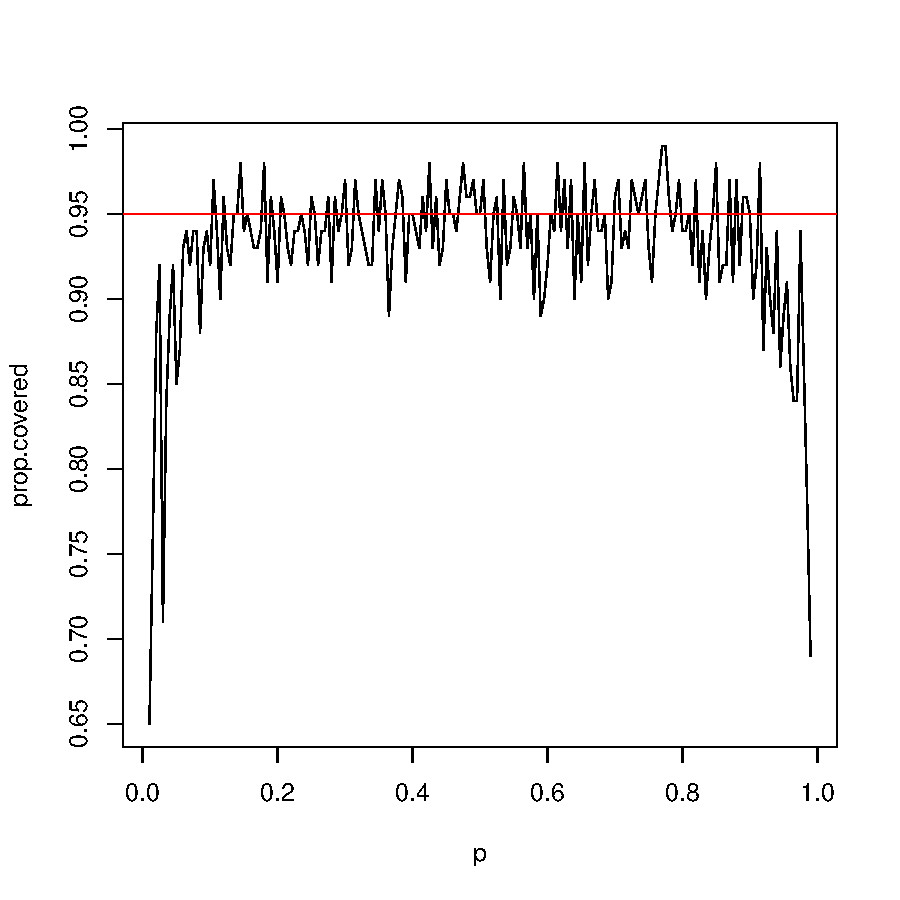
\includegraphics{sim_binomial_prop-010}

Die Frage, die sich hieran anschließt, ist ob sich neben der groben umgekehrten U-Form-Struktur weitere systematische Strukturen in der Verteilung verbergen. Hierzu wird eine erneute Analyse mit einer erhöhten Replikationszahl durchgeführt. 
 
\begin{Schunk}
\begin{Sinput}
> x <- p_study(100000, 100, .05, p.step=.005) 
> plot(x[c("p","prop.covered")], type="l") 
> abline(h=.95, col="red")
\end{Sinput}
\end{Schunk}
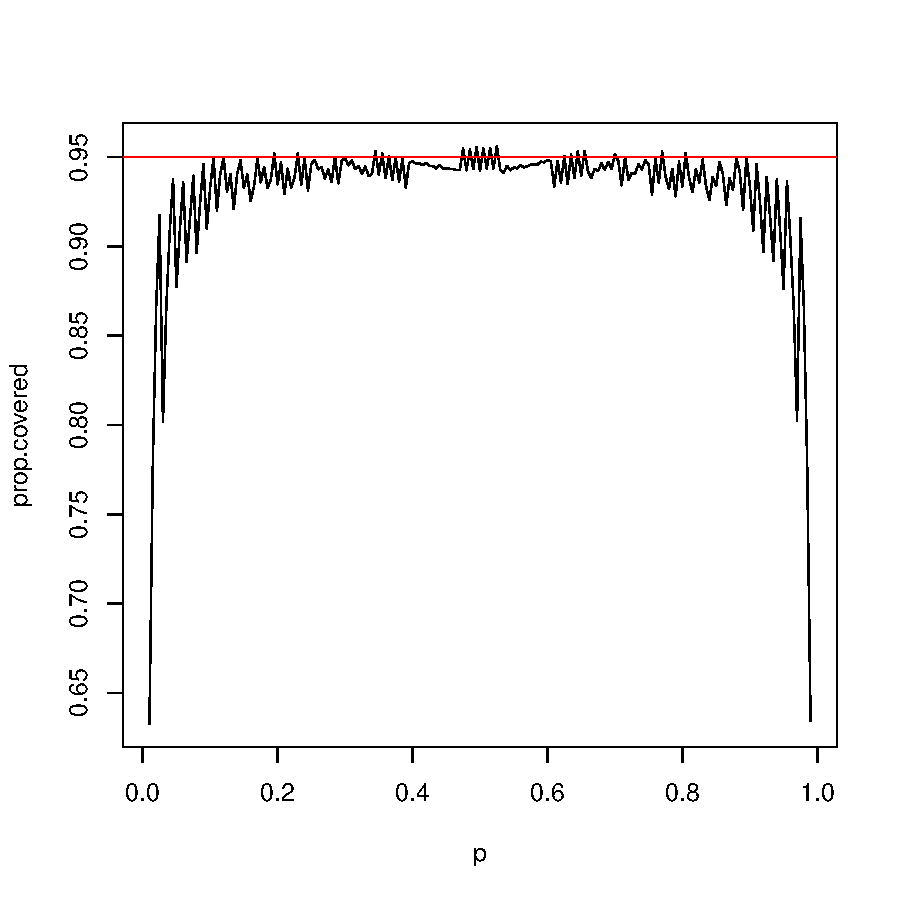
\includegraphics{sim_binomial_prop-013}

Es zeigt sich ein interessanter Effekt. Die Oszillationen der geschätzten Konfidenzintervalle in obiger Grafik ist keine Folge der geringen Replikationszahl sondern eine systematische Struktur.

Was lernen wir hieraus? Die Formel, die in viele Statistikbüchern enthalten ist, ist mit Vorsicht zu genießen, besonders bei Anteilswerten nahe $0$ oder $1$. Es gibt eine Reihe von Formeln mit besseren Eigenschaften, die später untersucht werden. Zum anderen zeigt sich eine spannende systematische Oszillation der geschätzeten Konfidenzintervalle, die wir auch bei anderen Schätzverfahren wiederfinden werden.

\textbf{Programmierung mittels Funktionen der \texttt{apply}-Familie}  

Als letzten Schritt soll demonstiert werden, wie der Code alternativ hätte geschrieben werden können. Hierzu nutzen wir anstelle von Schleifen Funktionen aus der \texttt{apply}-Familie. Der Code wird hierdurch i.d.R. kürzer. Auch führt die Nutzung von Funktionen aus der \texttt{apply}-Familie anstelle von Schleifen häufig zu einem Performancegewinn. Der Nachteil ist jedoch, dass sie am Anfang schwerer zu verstehen sind als Schleifen.
 
\begin{Schunk}
\begin{Sinput}
> sim_many_ci_2 <- function(reps, n, p, alpha=.05){
   res <- replicate(reps, sim_one_ci(n, p, alpha))
   prop.covered <- mean(res["covered", ])
   c(p=p, n=n, prop.covered=prop.covered)                   
 } 
> p_study_2 <- function(reps, n, alpha=.05,
                       p.start=.01, p.end=.99, p.step=.1){
   ps <- seq(p.start, p.end, p.step)                     
   res <- mapply(sim_many_ci_2, reps=reps,
                 n=n, p=ps, alpha=alpha)   
   as.data.frame(t(res))
 }   
> 
\end{Sinput}
\end{Schunk}

\par
\textbf{Erweiterung auf mehrere Formeln zur Schätzung der Konfidenzintervalle}  

Aufgrund der Probleme von Formel \ref{eq:prop_standard} sind in der Literatur weitere Ansätze zur Schätzung der Konfidenzintervalle für binomiale Anteile vorgeschlagen worden. Ein früher Ansatz stammt von Wilson (1927). Er schlägt folgende Intervalle vor. 

\begin{equation}  \label{eq:ci_wilson}
  p_{o,u} = \frac{1}{1 + \frac{c^2}{n}} \cdot \left(\hat p + \frac{c^2}{2n} \pm c\cdot\sqrt{\frac{\hat p \cdot (1-\hat p)}{n}+\frac{c^2}{4n^2}} \, \right)  
\end{equation}

Setzen wir diese Formel zunächst in eine \R{}-Funktion um.

\begin{Schunk}
\begin{Sinput}
> ci_wilson <- function(p.hat, n, alpha=.05){
   c <- qnorm(1 - alpha/2)
   pm <- c* sqrt(p.hat * (1 - p.hat)/n + c^2/(4*n^2))   
   c(p.hat= p.hat,
     lower= 1 / (1 + c^2/n) * (p.hat + c^2/(2*n) - pm),
     upper= 1 / (1 + c^2/n) * (p.hat + c^2/(2*n) + pm))
 } 
> ci_wilson(p.hat=.05, n=500)
\end{Sinput}
\begin{Soutput}
     p.hat      lower      upper 
0.05000000 0.03409375 0.07276816 
\end{Soutput}
\end{Schunk}

Wir wollen nun obige Analyse mit dem Wilson-Intervall wiederholen. Da wir dies zu Beginn nicht bedeacht haben, dass es mehrere Schätzverfahren gibt, sind wir gezwungen unseren Code umzuschreiben, um verschiedene Varianten einbeziehen zu können. Zur Programmierung gehen wir von der Überlegung aus, dass die Parameter die an die Funktionen übergeben werden stets $n$, $p.hat$ und $alpha$ sein werden. Wir schreiben nun eine Funktion, die das Argument \texttt{method} enthält. Über dieses kann das gewünschte Verfahren ausgewählt werden. Die Funktion match.arg sorgt hierbei dafür, dass es auch möglich ist, den Namen der Methode teilweise auszuschreiben. Wenn diese zeile weggelassen wird, müsste die Methode stets exakt benannt werden.

\begin{Schunk}
\begin{Sinput}
> ci <- function(p.hat, n, alpha=.05, method="standard"){
   method <- match.arg(method, c("standard", "wilson"))  
   if (method == "standard")
     res <- ci_standard(p.hat, n, alpha)
   if (method == "wilson")       
     res <- ci_wilson(p.hat, n, alpha)
   res
 }   
\end{Sinput}
\end{Schunk}

Erweitern wir nun unsere vorherigen Funktionen auch um das Argument \texttt{method} und ersetzen die Funktionen zur Berechnung der Konfidenzintervalle mit der Funktion \texttt{ci}.

\begin{Schunk}
\begin{Sinput}
> sim_one_ci <- function(n, p, alpha=.05, 
                         method="standard"){
   vals <- rbinom(n, 1, p)                # Stichprobe ziehen 
   p.hat <- mean(vals)                    # geschätzter Anteil 
   cis <- ci(p.hat, n, alpha, method)     # KI berechnen
   lower <- cis[["lower"]]                # unteres KI
   upper <- cis[["upper"]]                # oberes KI  
   c(p.hat=p.hat,                         # Punktschätzung
     lower= lower, upper= upper,          # KI ausgeben   
     covered= lower <= p && p <= upper)   # liegt p im Intervall?
 }
> sim_many_ci <- function(reps, n, p, alpha=.05,
                           method="standard"){
   res <- replicate(reps, sim_one_ci(n, p, alpha, method))
   prop.covered <- mean(res["covered", ])
   c(p=p, n=n, prop.covered=prop.covered)                   
 } 
> p_study <- function(reps, n, alpha=.05, method="standard",
                       p.start=.01, p.end=.99, p.step=.1){
   method <- match.arg(method, c("standard", "wilson"))  
   ps <- seq(p.start, p.end, p.step)                     
   res <- mapply(sim_many_ci, reps=reps,
                 n=n, p=ps, alpha=alpha, method=method)   
   df <- as.data.frame(t(res))
   df$method <- method
   df
 } 
\end{Sinput}
\end{Schunk}
 
Nun können wir obige Analyse für zwei Schätzverfahren durchführen. Ergänzen wir die Untersuchung nun um das Wilson-Intervall, diesmal direkt mir einer großen Replikationszahl.

\begin{Schunk}
\begin{Sinput}
> x <- p_study(100000, 100, .05, p.step=.01, method="wilson")
> plot(x[c("p","prop.covered")], type="l", las=1) 
> abline(h=.95, col="red")
\end{Sinput}
\end{Schunk}


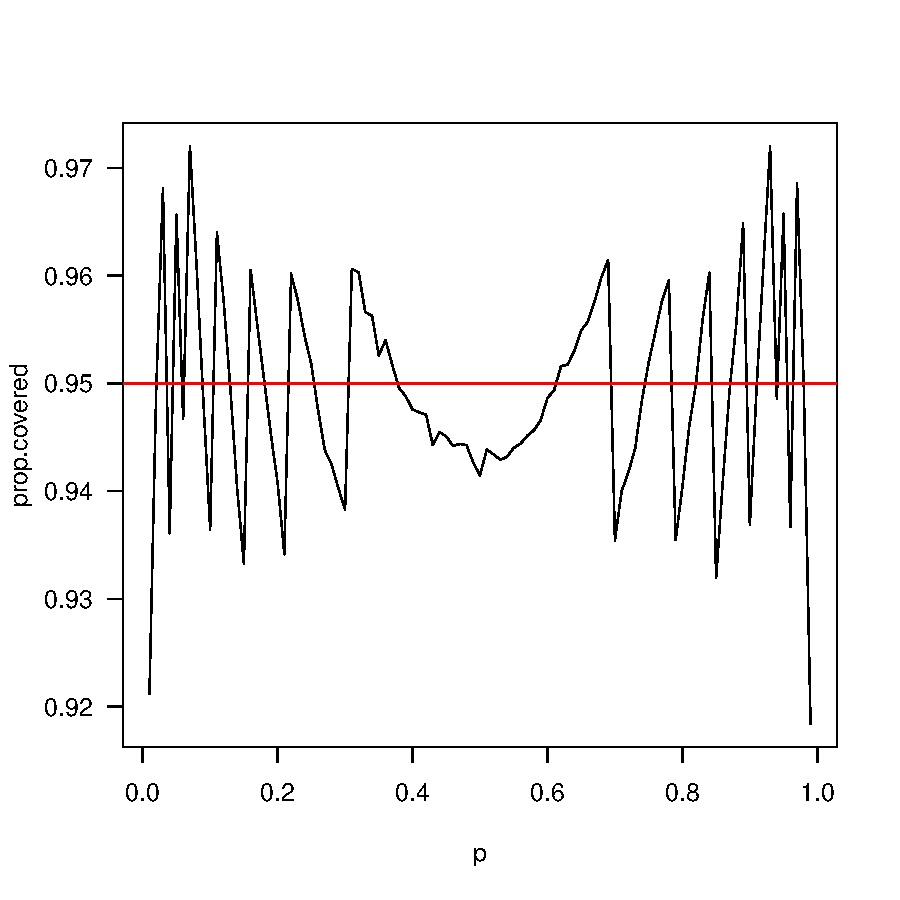
\includegraphics{sim_binomial_prop-020}

Es zeigt sich, dass die Werte deutlich dichter um $95\%$ schwanken, als bei der Standardvariante. Jedoch sind auch diese Ergebnisse keinesfalls befriedigend. Es existieren weitere Varianten, z.\,B. im Paket \texttt{binom}, die bessere Ergebnisse liefern.


\textbf{Untersuchung weiterer Parameter} 

Bisher haben wir das Verhalten des Konfidenzintervalls lediglich durch die Variation von $p$ untersucht. Die zweite Variable innerhalb der Gleichung ist $n$. Im Folgenden soll die Simulation für verschiedene $n$ und $p$ durchgeführt werden. Hierzu wird eine leere Liste angelegt, in der die Ergebnisse für jedes $n$ gespeichert werden. Die letzte Zeile verbindet die Dataframes aus den einzelnen Listenelementen zu einem großen Dataframe.

\begin{Schunk}
\begin{Sinput}
> res <- list()
> ns <- 10:100
> for (i in seq_along(ns)){
   cat(paste("\r", "run", i, "of", length(ns)))
   res[[i]] <- p_study(reps=10, n=ns[i], p.step=.1, 
                       method="standard")
 } 
> x <- do.call(rbind, res)
\end{Sinput}
\end{Schunk}

% <<eval=F>>=   
% write.csv2(x, file="data/p_study_standard_05_n100_reps1000.csv")
% @   
    

Um die Daten zu visualisieren wird die Funktion \texttt{levelplot} aus dem \texttt{lattice} Paket genutzt.
  
\begin{Schunk}
\begin{Sinput}
> library(lattice)
> levelplot(prop.covered ~ n * p, data=x)
\end{Sinput}
\end{Schunk}

Diese Visualisierung ist verbesserungsbedürftig. Uns interessiert besonders der Bereich einer Überdeckungswahrscheinlichkeit zwischen $.8$ und $1.0$. Weiterhin sollen Werte über $.95$ grüne und unterhalb rote Farben ausfweisen. Zum Erzeugen einer Farbpalette wird die Funktion \texttt{colorpanel} aus dem Paket \texttt{qplot} genutzt. 

\begin{Schunk}
\begin{Sinput}
> library(gplots)
> library(lattice) 
> levels <- seq(.8, 1, by=.05)
> colors <- c(colorpanel(4, "darkred", "red"), "lightgreen")
> levelplot(prop.covered ~ n * p, data=x, 
            at=levels, col.regions=colors)            
\end{Sinput}
\end{Schunk}
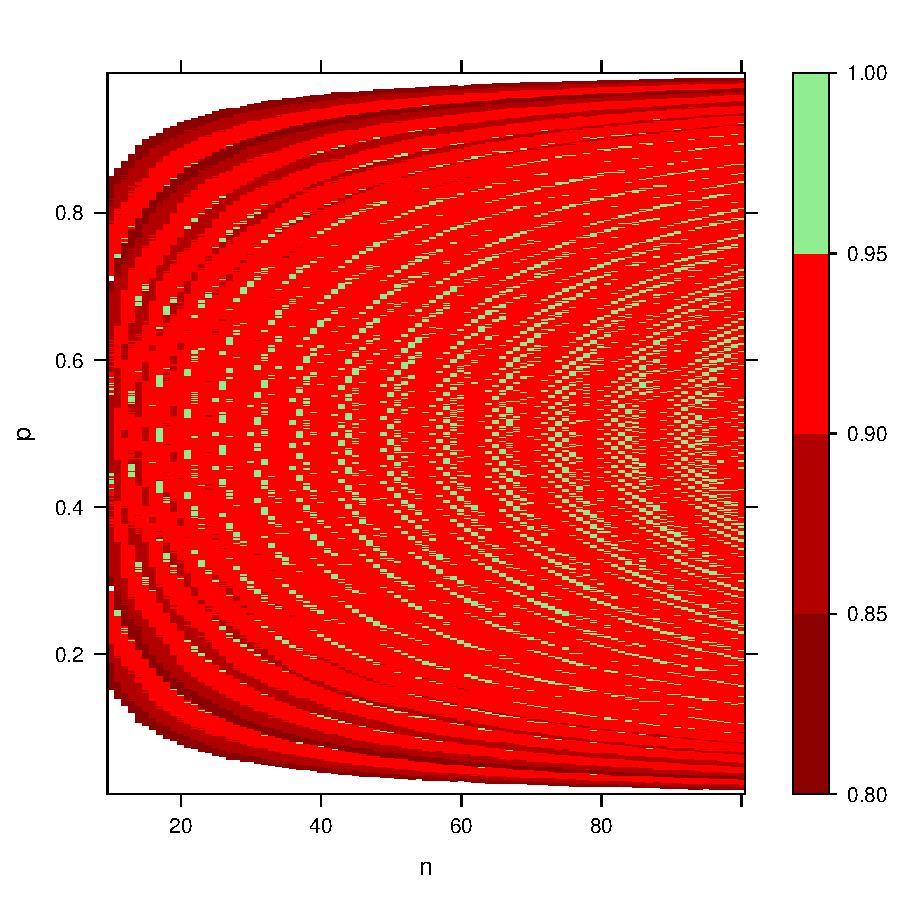
\includegraphics{sim_binomial_prop-024}

Die Grafik zeigt, dass die Performance der Formel mit steigendem $n$ in den Randbereichen von $p$ besser wird. Das oszillierende Muster bleibt jedoch auch bei größerem $n$ erhalten.


\begin{Schunk}
\begin{Sinput}
> levels <- seq(.8, 1, by=.05)
> colors <- c(colorpanel(4, "darkred", "red"), "lightgreen")
> levelplot(prop.covered ~ n * p, data=x, 
            at=levels, col.regions=colors)            
\end{Sinput}
\end{Schunk}
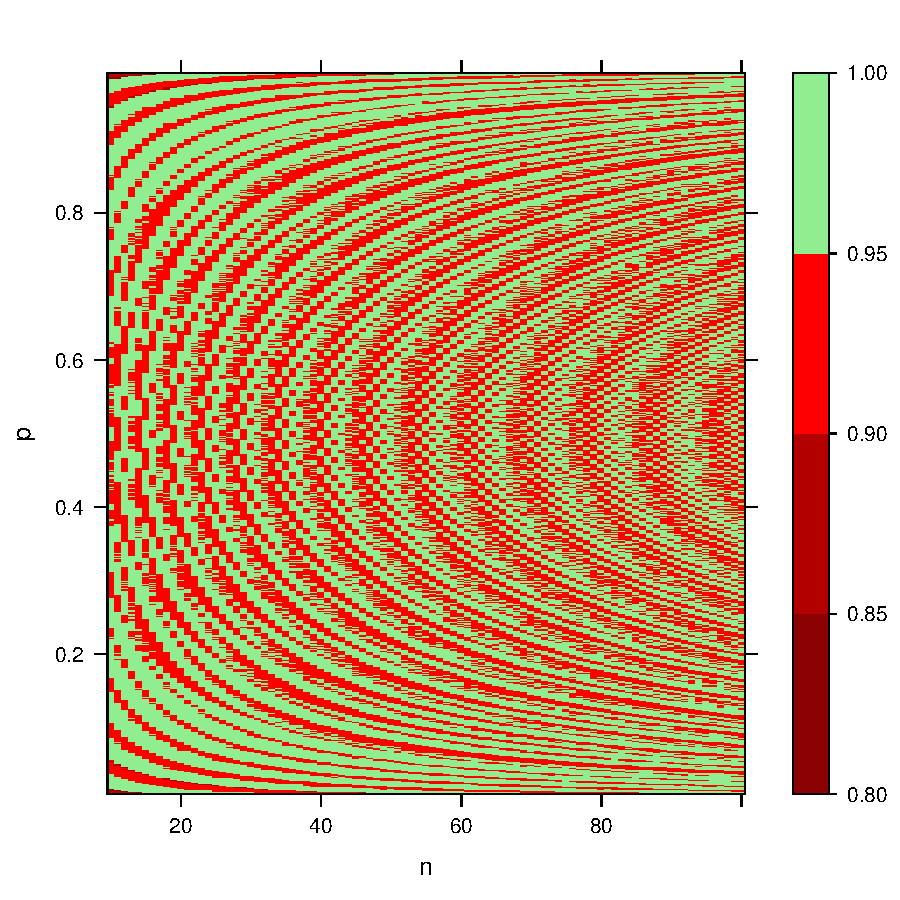
\includegraphics{sim_binomial_prop-026}

% <<>>=
% contourplot(prop.covered ~ n * p, data=x, 
%            at=levels, labels=F, region=T, col.regions=colors)
% @ 
% <<eval=F, echo=F>>=
% # alternative code
% library(gplots)
% library(reshape2)
% y <- acast(x, n ~ p, value.var="prop.covered")
% levels <- seq(.8, 1, by=.01)
% greens <- colorpanel(6, "darkgreen", "lightgreen")
% reds <- colorpanel(15, "darkred", "red")
% colors <- c(reds, greens)
% labels <- seq(10, 40, by=5)
% plot.axes <- function(){
%   axis(1, at=(labels-10)/(40-10), labels=labels)
%   axis(2)
% }
% filled.contour(y, levels=levels, nlevels=11, col=colors)#, plot.axes=plot.axes())  
% @

%%%%%%%%%%%%%%%%%%%%%%%%%%%%%%%%%%%%%%%%%%%%%%%%%%%%%%%%%%%%%%%%%%%%%%%%%%%%%%%
 
\newpage  
                             %%%%%%%%%%%%%%%%%%%%%%%%%%%%%%%%%%%%%%%%%%%%%%%%%%%%%%%%%%%%%%%%%%%%%%%%%%%%%%%
%%% SWEAVE
       % Ihaka, R. (2009). Customizing Sweave 
%%%%%%%%%%%%%%%%%%%%%%%%%%%%%%%%%%%%%%%%%%%%%%%%%%%%%%%%%%%%%%%%%%%%%%%%%%%%%%%
%%% CUSTOMIZING SWEAVE 
%%% from: Ihaka, R. (2009). Customizing Sweave to Produce Better Looking LATEX Output
\DefineVerbatimEnvironment{Sinput}{Verbatim}{fontsize=\footnotesize, formatcom=\color{codecolor}, xleftmargin=2em}
\DefineVerbatimEnvironment{Soutput}{Verbatim}{fontsize=\footnotesize, xleftmargin=2em, formatcom=\color{codecolor}} 
\DefineVerbatimEnvironment{Scode}{Verbatim}{fontsize=\footnotesize, xleftmargin=2em, formatcom=\color{codecolor}}

\renewenvironment{Schunk}{\vspace{10pt}}{\vspace{8pt}}   
%%%%%%%%%%%%%%%%%%%%%%%%%%%%%%%%%%%%%%%%%%%%%%%%%%%%%%%%%%%%%%%%%%%%%%%%%%%%%%%
%%%%%%%%%%%%%%%%%%%%%%%%%%%%%%%%%%%%%%%%%%%%%%%%%%%%%%%%%%%%%%%%%%%%%%%%%%%%%%%

\section{Compare true sequences of coins flips and made up ones}

Vergleich von zufälligen binären Matrizen und willentlich erzeugten, die durch 
Menschen tendieren dazu, die Anzahl an langen identischen Strecken von gleichen Zahlen zu unterschätzen und die Anzahl an Wechseln zu überschätzen. 
     
Wir brauchen:
1) Die Anzahl an Wechseln
2) Längste Sequenz 

\begin{Schunk}
\begin{Sinput}
> # ok
> coin_runs <- function(n){
   x <- rbinom(n, 1, .5)
   re <- rle(x)$length
   c(flips=length(re) - 1, max=max(re))  
 }
> coin_runs(100)
\end{Sinput}
\begin{Soutput}
flips   max 
   45     8 
\end{Soutput}
\begin{Sinput}
> # repeat a large number of times  
> # using a for loop
> do_coin_runs <- function(reps, n=100){
   res <- matrix(NA, reps, 2)
   for (i in 1:reps)
     res[i, ] <- coin_runs(n)
   res <- as.data.frame(res)
   names(res) <- c("flips", "max")
   res
 }
> do_coin_runs(10)  
\end{Sinput}
\begin{Soutput}
   flips max
1     50   7
2     49   7
3     45   6
4     49   7
5     46  11
6     45   9
7     51   6
8     47   7
9     48   8
10    50   8
\end{Soutput}
\begin{Sinput}
> # much simpler: using replicate  
> do_coin_runs_2 <- function(reps, n=100){
   as.data.frame(t(replicate(reps, coin_runs(n))))
 } 
> x <- do_coin_runs_2(10000) 
> colMeans(x)
\end{Sinput}
\begin{Soutput}
  flips     max 
49.4137  6.9712 
\end{Soutput}
\begin{Sinput}
> do_coin_plot <- function(df){ 
   x <- df[, 1]
   y <- df[, 2]
   plot(jitter(x), jitter(y), pch=16, cex=.2, col="darkblue", 
        xlab="flips", ylab="longest run") 
   grid()
 } 
> 
\end{Sinput}
\end{Schunk}

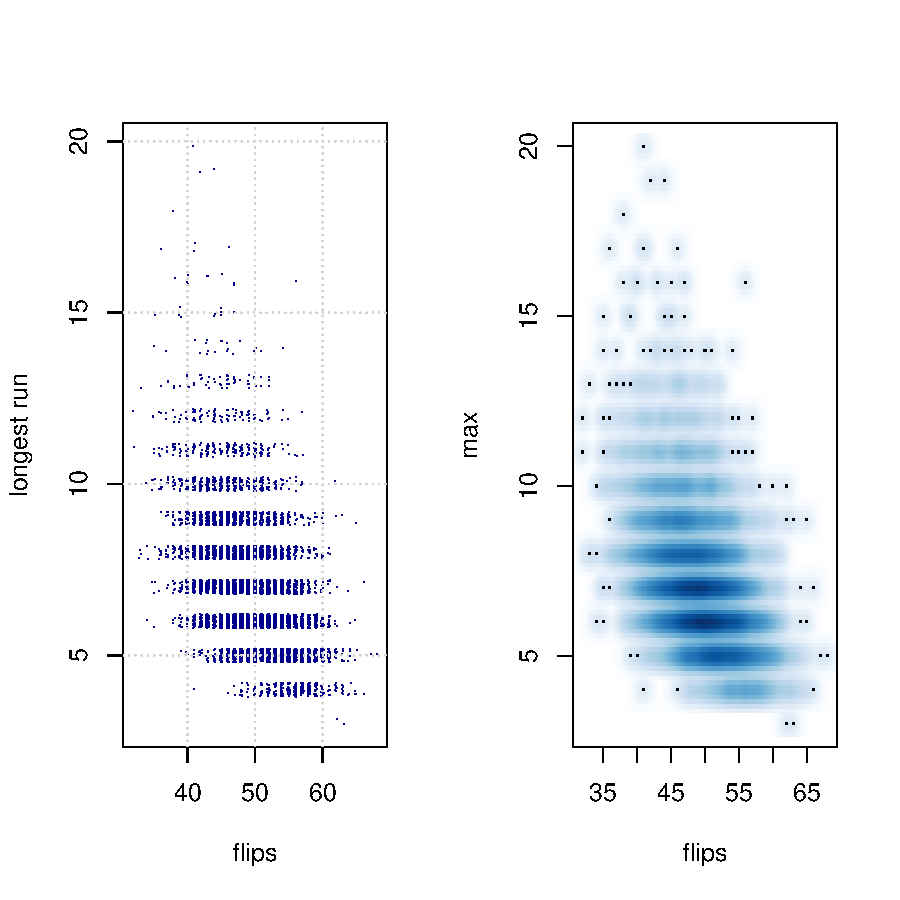
\includegraphics{sim_coinflips-003}

%%%%%%%%%%%%%%%%%%%%%%%%%%%%%%%%%%%%%%%%%%%%%%%%%%%%%%%%%%%%%%%%%%%%%%%%%%%%%%%
 
\newpage
\include{sim_monty_hall} 
\newpage
                             %%%%%%%%%%%%%%%%%%%%%%%%%%%%%%%%%%%%%%%%%%%%%%%%%%%%%%%%%%%%%%%%%%%%%%%%%%%%%%%
%%% SWEAVE
       % Ihaka, R. (2009). Customizing Sweave 
%%%%%%%%%%%%%%%%%%%%%%%%%%%%%%%%%%%%%%%%%%%%%%%%%%%%%%%%%%%%%%%%%%%%%%%%%%%%%%%
%%% CUSTOMIZING SWEAVE 
%%% from: Ihaka, R. (2009). Customizing Sweave to Produce Better Looking LATEX Output
\DefineVerbatimEnvironment{Sinput}{Verbatim}{fontsize=\footnotesize, formatcom=\color{codecolor}, xleftmargin=2em}
\DefineVerbatimEnvironment{Soutput}{Verbatim}{fontsize=\footnotesize, xleftmargin=2em, formatcom=\color{codecolor}} 
\DefineVerbatimEnvironment{Scode}{Verbatim}{fontsize=\footnotesize, xleftmargin=2em, formatcom=\color{codecolor}}

\renewenvironment{Schunk}{\vspace{10pt}}{\vspace{8pt}}   
%%%%%%%%%%%%%%%%%%%%%%%%%%%%%%%%%%%%%%%%%%%%%%%%%%%%%%%%%%%%%%%%%%%%%%%%%%%%%%%
%%%%%%%%%%%%%%%%%%%%%%%%%%%%%%%%%%%%%%%%%%%%%%%%%%%%%%%%%%%%%%%%%%%%%%%%%%%%%%%

\section{Prisoner problem}

Drei Türen. Wir wissen nciht welche welche ist. 
 
\begin{itemize}
\item Tür 1 führt zur Freiheit
\item Tür 2 zur weiteren 2 Stunden im Meeting und danach wieder zum Anfang der Situation  
\item Tür 3 zur weiteren 5 Stunden im Meeting und danach wieder zum Anfang der Situation 
\end{itemize} 

Wie lange dauert es im Schnitt zur Freiheit? Die Schritte werden weiderholt, bis man die erste Tür gewählt hat.

\begin{Schunk}
\begin{Sinput}
> # prisoner walk
> prisoner <- function(p=c(1/3, 1/3, 1/3), penalty=c(0,2,5)){
   penalty.sum <- 0
   door <- 0
   while(door != 1){
     door <- sample(1:length(p), 1)
     penalty.sum <- penalty.sum + penalty[door]    
   }
   penalty.sum  
 }      
> prisoner()
\end{Sinput}
\begin{Soutput}
[1] 5
\end{Soutput}
\begin{Sinput}
> sim_prisoner <- function(reps=1000, p=c(1/3, 1/3, 1/3), 
                          penalty=c(0,2,5), do.plot=TRUE){
   res <- rep(NA, reps)
   for (i in 1:reps)
     res[i] <- prisoner(p, penalty)
   mn <- mean(res)    
   if (do.plot){   
     h <- hist(res, col="lightgrey", xlab="Hours", breaks=15)
     abline(v=mn, col="red")
     text(mn, max(h$counts)/2, paste("expected value=", mn), pos=4)  
   }
   res
 }
\end{Sinput}
\end{Schunk}

\begin{Schunk}
\begin{Sinput}
> dummy <- sim_prisoner() 
\end{Sinput}
\end{Schunk}
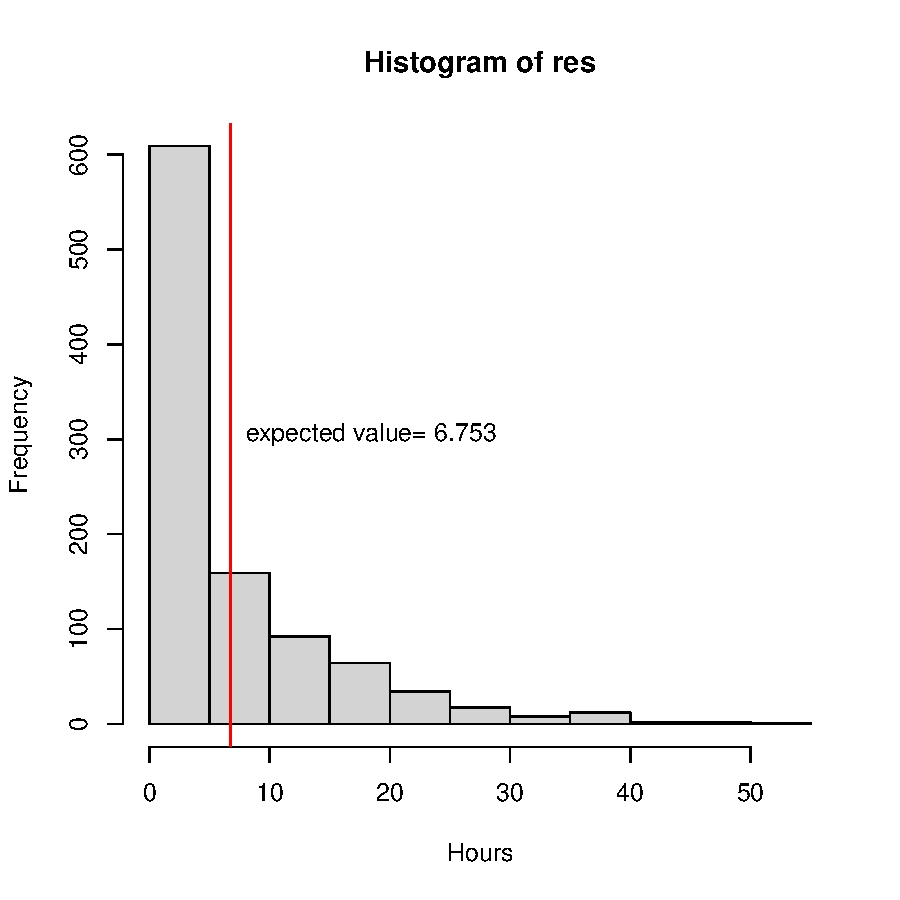
\includegraphics{sim_prisoner_problem-003}


%%%%%%%%%%%%%%%%%%%%%%%%%%%%%%%%%%%%%%%%%%%%%%%%%%%%%%%%%%%%%%%%%%%%%%%%%%%%%%%
 
\newpage
\section*{Literature}
\addcontentsline{toc}{section}{Literature}

% alternatively if not hangpars environment:
% \hangindent+10mm %\hangafter=1 
% in front of each paragraph

% \begin{hangparas}{.25in}{1}
% Hartmann, A. (1992). Element Comparisons In Repertory Grid Technique: Results And Consequences Of A Monte Carlo Study. {\it International Journal of Personal Construct Psychology, 5}(1), 41-56.
% 
% Slater, P. (1977).{\it The measurement of intrapersonal space by Grid technique: Dimensions of intrapersonal space.}  (Vol. 2). London: Wiley \& Sons.
% \end{hangparas} 

\end{document}

